\documentclass[12pt]{article}
\usepackage{mdframed} % tb pour marep
\usepackage{comment} % pour l'affichage conditionnel
\usepackage{graphicx} % images
\usepackage{float} % option H dans figure

\newif\ifDispRep
%\DispReptrue  % Show the text
\DispRepfalse % Hide the text

\newmdenv[linecolor=black]{tb}

\ifDispRep
\newenvironment{MaReponse}{\begin{tb}}{\end{tb}}
\else
\excludecomment{MaReponse}
\fi

\newcommand{\MaQuest}[1]{\par\vspace{0.3\baselineskip}\noindent$\rightarrow$\textit{#1}\par\vspace{0.3\baselineskip}}

\begin{document}
	
	Bonjour
	\MaQuest{Q1}
	Suite
	\begin{MaReponse}
		\begin{figure}[H]
			\centering
			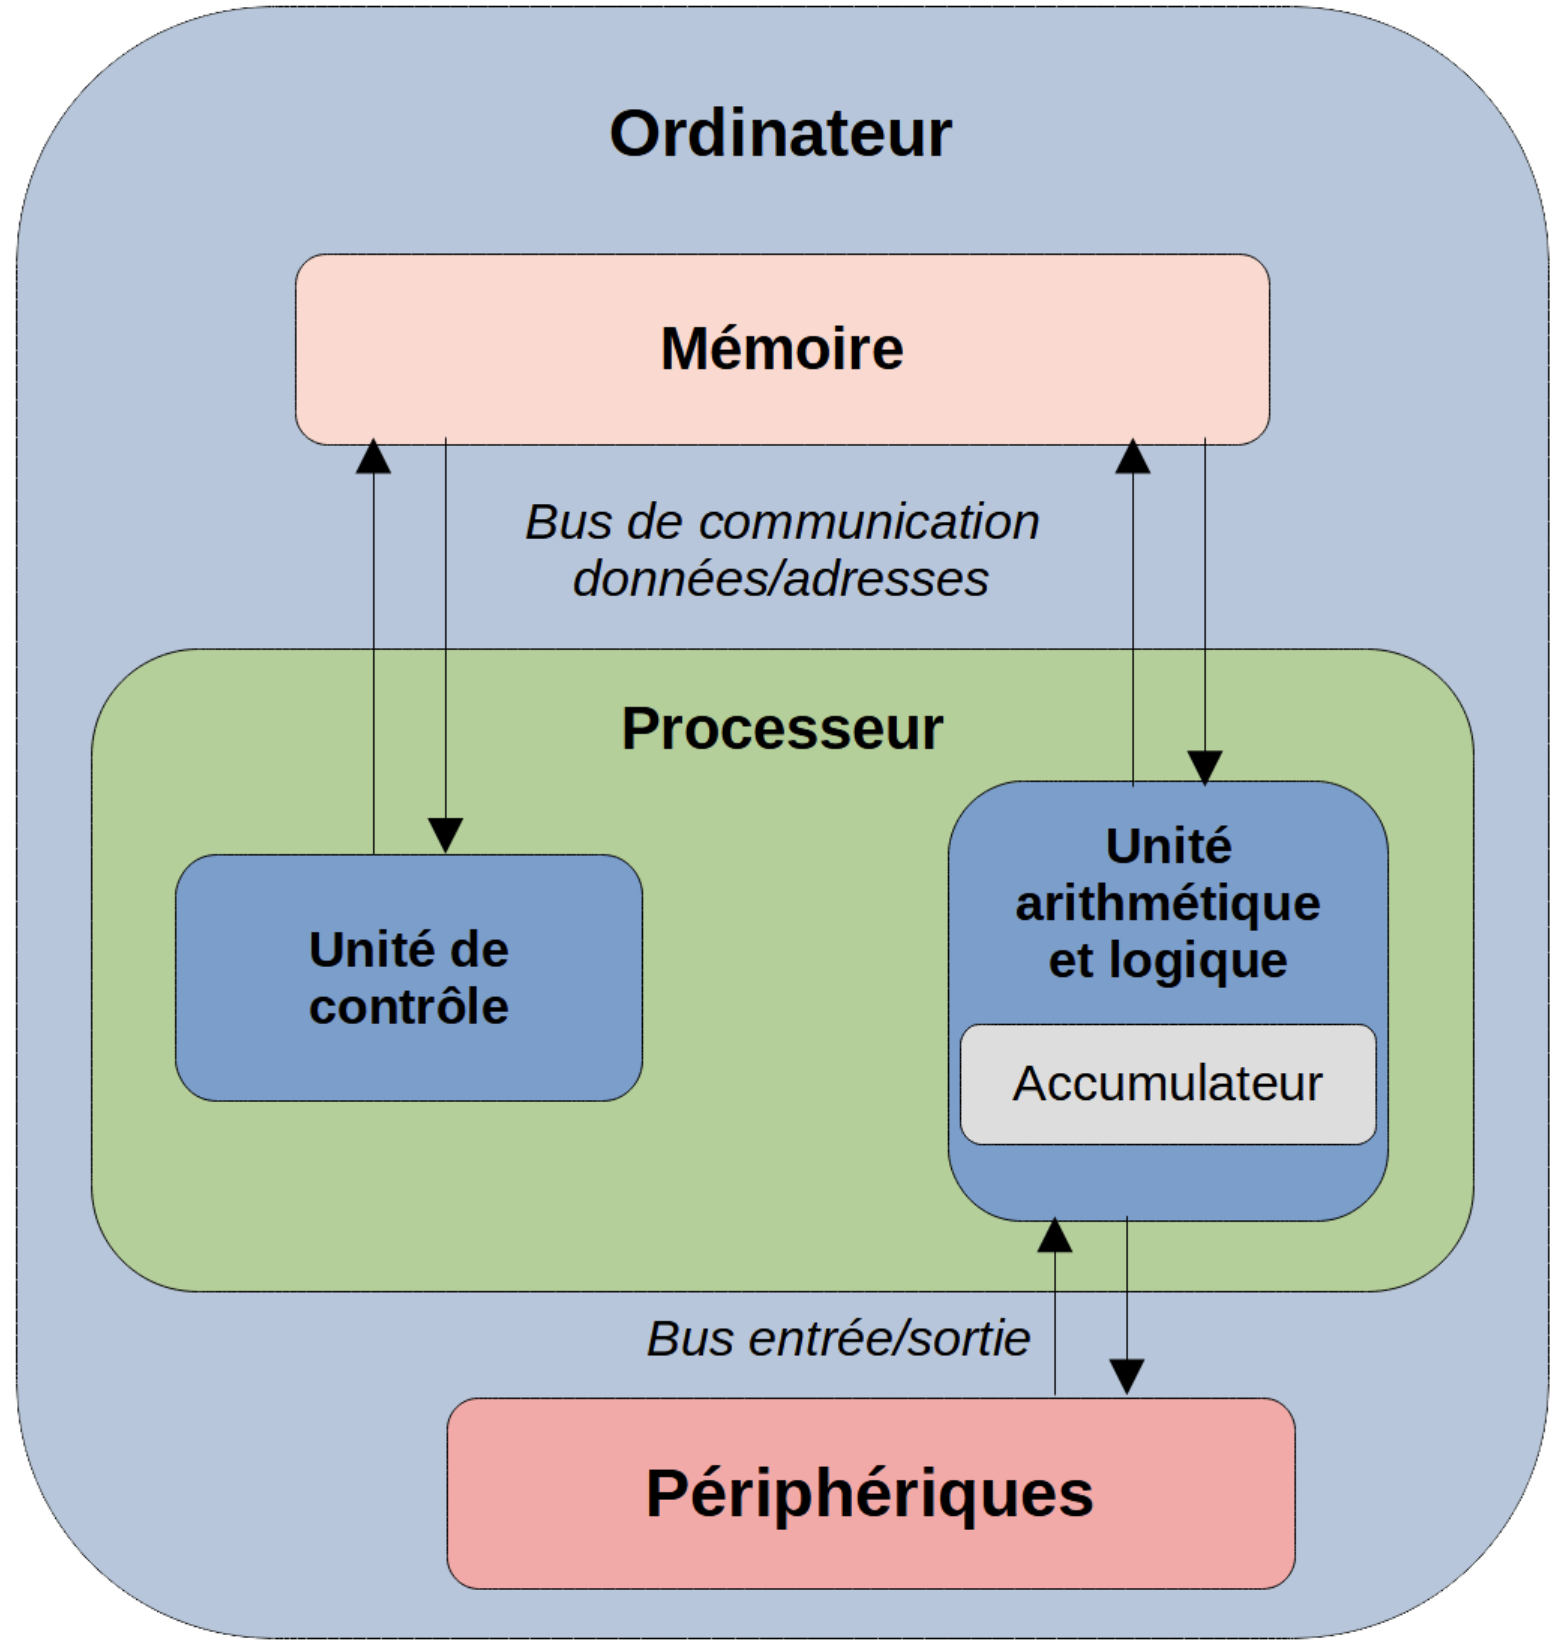
\includegraphics[width=0.5\textwidth]{002_VonNeumann.png}
		\end{figure}
		R1
	\end{MaReponse}
	Fin
\end{document}
